\documentclass[portrait, a0, 30pt]{sciposter}
\usepackage[scaled=0.84]{helvet}
\usepackage{multicol, caption}
\usepackage[british]{babel}
\usepackage[utf8]{inputenc}
\usepackage{graphicx}
\usepackage{natbib}
\usepackage{times}
\usepackage{amsmath}
\usepackage{mathtools}
\usepackage{amsfonts}
\usepackage{verbatim}
\usepackage{graphicx}
\usepackage{framed}
\usepackage{xcolor}

\setcitestyle{authoryear,open={[},close={]}}

\DeclareMathOperator*{\argmax}{arg\,max}
\DeclareMathOperator*{\argmin}{arg\,min}

\DeclareMathOperator*{\KL}{{\rm KL}}
\DeclareMathOperator*{\const}{{\rm const}}

\colorlet{shadecolor}{lightgray!30}

\author{William van Rooij\\ \textit{\normalsize Master thesis supervised by Hélène Ruffieux and Anthony Davison}}
\title{Averaged Variational Inference for Hierarchical Modelling of Genetic Association}
\leftlogo{images/EPFL_logo}
\date{July 2019}
\institute{École Polytechnique Fédérale de Lausanne, Lausanne, Switzerland}

\renewcommand{\titlesize}{\huge}
\renewcommand{\baselinestretch}{1.2}

\begin{document}
\maketitle
\begin{multicols*}{2}
\section{Introduction}
In \textbf{genome-wide association studies} (GWAS), we estimate the associations between \textbf{single nucleotide polymorphisms} (SNPs) and a phenotype or \textbf{trait}. It is a \textit{small n, large p} situation where
\begin{itemize}
\item $n$ is the number of observations,
\item $p$ is the number of SNPs.
\end{itemize}
In a \textit{small n, large p} situation, traditional Bayesian inference methods such as \textbf{Markov Chain Monte Carlo} (MCMC) algorithms often scale poorly. An alternative is to use \textbf{variational inference} \citep{varInf}.

Moreover, SNPs data are often highly correlated with a block structure, which complicates inference and interpretation. Here, we seek to enhance regression approaches in such difficult settings.



\section{Hierarchical Regression Model}
Let $\boldsymbol{X} = (X_1,\dots,X_p)$ represent the SNPs, and $\boldsymbol{y}$ represent the trait observed.

$\boldsymbol{y}$ is linearly related with the predictors $\boldsymbol{X}$ and has residual precision $\tau$. We suppose that they follow the following hierarchical model,
\begin{align*}
\boldsymbol{y} \mid \boldsymbol{\beta}, \tau &\sim\mathcal{N}\left(\boldsymbol{X\beta}, \tau^{-1}\boldsymbol{I}_n\right),\\
\beta_s \mid \gamma_s, \tau, \sigma^{-2} &\sim \gamma_s\;\mathcal{N} \left( 0, \sigma^2 \tau^{-1} \right) + (1-\gamma_s)\;\delta_0,\\
\gamma_s \mid \omega_s &\sim \mathrm{Bernoulli}\left(\omega_s\right),\\
\omega_s &\sim \mathrm{Beta}\left(a_s, b_s\right),
\end{align*}
for all $s = 1,\dots , p$, where $\delta_0$ is the Dirac distribution, and $a_s$ and $b_s$ are chosen to enforce sparsity \citep{eff_inf}. $\boldsymbol{\gamma}$ is a binary vector that that indicates which SNP is associated with the trait, i.e.,
\begin{center}
$\gamma_s = 1 \Longleftrightarrow$ SNP $ s $ is associated with the trait.
\end{center}
\section{Variational Inference}
Given a family of densities $\mathcal{D}$ over the parameters $\boldsymbol{\theta}$, variational inference approximates the density of interest $p(\boldsymbol{\theta}\mid\boldsymbol{y})$ by a distribution $q \in \mathcal{D}$ that minimizes the ``reverse'' \textbf{Kullback--Leibler divergence},
\begin{equation*}
\KL (q \parallel p) = \int q(\boldsymbol{\theta}) \log \left\lbrace\frac{q(\boldsymbol{\theta})}{p(\boldsymbol{\theta}\mid\boldsymbol{y})}\right\rbrace.
\end{equation*}

We introduce the \textbf{evidence lower bound},
\[
\mathcal{L}(q)=\mathbb{E}_q\left[\log p(\boldsymbol{\theta},\boldsymbol{y})\right]-\mathbb{E}_q\left[\log q(\boldsymbol{\theta})\right] = \int q(\boldsymbol{\theta})\log\frac{p(\boldsymbol{y},\boldsymbol{\theta})}{q(\boldsymbol{\theta}}\mathrm{d}\boldsymbol{\theta},
\]
where $\mathbb{E}_q$ represents the expectation with respect to $q$.

The lower bound verifies
\[
\KL(q\parallel p) = \log(p)-\mathcal{L}(q).
\]

As the Kullbak--Leibler divergence can be difficult to minimize, variational inference maximizes the lower bound instead.

\begin{shaded}
When applied to highly correlated data, variational inference \textbf{underestimates} posterior variances,this is a consequence of: \begin{itemize}
\item the \textbf{high multimodality} of the lower bound $\mathcal{L}(q)$,
\item the \textbf{mean-field independence} assumption,
\item the \textbf{reverse Kullback--Leibler} divergence optimisation,
\end{itemize}
and results in a tendency for the approximation to concentrate mass on a single mode and report a set of predictors with very high confidence.

To better handle the multimodality, we build a method consisting of averaging over multiple runs with different parameter initialisations with weights equal to the posterior model probability.
\end{shaded}
\columnbreak
\section{Averaged LOCUS method}
Assume that the data $\boldsymbol{y}$ has been obtained from a one of $K$ models $M_k,\quad k=1,\dots,K$. We want to estimate the associations between the SNPs and the trait.

We perform a weighted average accounting for the likelihood that the data corresponds to each model, i.e., for all $s = 1,\dots,p$, 
\begin{equation*}
\mathbb{E}\left[\gamma_s\mid \boldsymbol{y}\right] = \sum_{k=1}^K\mathbb{E}\left[\gamma_s\mid M_k, \boldsymbol{y}\right]\;p(M_k\mid \boldsymbol{y}).
\end{equation*}
The posterior probability for model $M_k$ is 
\begin{equation*}
p(M_k\mid \boldsymbol{y}) = \frac{p(\boldsymbol{y}\mid M_k)\;p(M_k)}{\sum_{j=1}^K p(\boldsymbol{y}\mid M_j)\; p(M_j)} \approx \frac{\exp\left\lbrace\mathcal{L}(q)\right\rbrace\; p(M_k)}{\sum_{j=1}^K \exp\left\lbrace\mathcal{L}(q)\right\rbrace\; p(M_j)}
\end{equation*}
where $p(\boldsymbol{y}\mid M_k)$ is the likelihood under model $M_k$, approximated by $\exp\left\lbrace\mathcal{L}(q)\right\rbrace$, and $p(M_k)$ is the prior probability of model $M_k$.
\section{Performance}
We compare the performance of variable selection of five methods,
\begin{itemize}
\item classical variational algorithm ``LOCUS'', \citep{eff_inf},
\item averaged variational algorithm ``averaged LOCUS'',
\item their annealing augmented equivalents ``annealed LOCUS'' and ``averaged annealed LOCUS'',
\item averaged variational algorithm with equal weights ``averaged LOCUS (Equal weights)''
\end{itemize}

\begin{figure}[H]
\centering
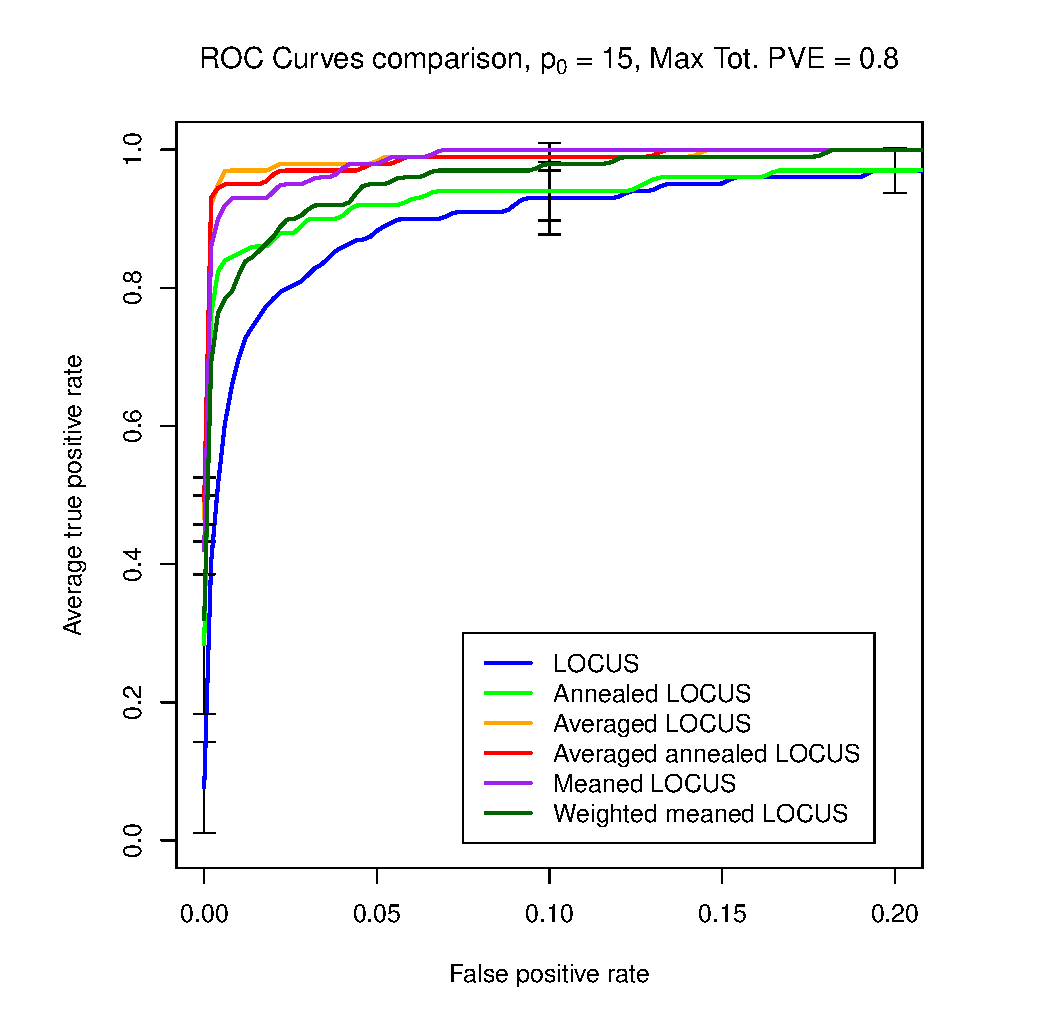
\includegraphics[width=11in]{images/ROC_curves.pdf}
\caption{\label{fig:ROC}Comparison of ROC curves between LOCUS, averaged LOCUS, their respective annealed versions, and averaged LOCUS with equal weights, colored in blue, orange, green, red, and purple respectively. The data involve $300$ observations, $15$ SNPs out of $500$ SNPs are associated with the trait. The response variance explained by the SNPs is below $80\%$.}
\end{figure}

The three averaging methods have similar variable selection performance, which is better than the standard LOCUS method. The annealing step only improves the performance of variable selection in the non-averaged cases.
\section{Conclusion}
The averaged variational inference better handles the multimodality of the posterior and better conveys the uncertainty due to the strong correlation structure in the data.

The averaged methods can be implemented in parallel, drastically diminishing the runtime.
\bibliography{references}
\bibliographystyle{apalike}
\end{multicols*}
\end{document}